\section{Overview of VTK-m}

\assign{Hank, editting pass (perhaps trimming)}

The origin of the VTK-m library \cite{Moreland2016} is a USDOE ASCR research project to enable scientific visualization on emerging HPC systems.
The main goals of VTK-m are twofold: to serve as a repository for interoperable scientific visualization algorithms well suited to accelerator architectures and to provide a framework that simplifies the development of visualization algorithms that can be ported across many accelerator devices.

\ken{Idea from Jay: summarize the filters and stuff we have done in a table so that people can easily add their work.}

\jay{Table is added and we might simplify this paragraph a little bit and put detailed references into the table.}

At the onset of ECP, VTK-m contained only the most common operations for scientific visualization: contour \cite{Lo2012}, threshold \cite{Maynard2013}, external faces \cite{Lessley2016}, basic surface simplification \cite{Moreland2016}, and rendering \cite{Larsen2015:VR,Larsen2015:RayTrace}.
Although this initial set covers much of the basic needs for scientific visualization, practitioners require much more functionality.
ECP was fundamental in growing this functionality with the introduction of many more algorithms.
Notably, these include clip, connectivity, clean grid, material interface reconstruction, statistics, gradients, density estimation, coordinate transformation, streamlines and other flow algorithms \cite{Pugmire2018}, surface normal generation, mesh quality metrics, resampling, and contour tree \ken{cite} as well as numerous optimizations.
These added features provide the necessary functionality for the tools and applications, discussed later in this paper, that rely on VTK-m to execute on Exascale machines and similar hardware.

VTK-m also internally provides a framework that simplifies the implementation of these and future algorithms as well as ports these algorithms across different devices.
The basic structure of the framework is shown in Figure~\ref{fig:vtkm-framework}.
Code in VTK-m is separated into two separate environments: control and execution.
These correspond to the ``host'' and ``device,'' respectively, in a GPU development environment.
That said, the logical control and execution environments are maintained even when there is not a clear separation between host and device, which is the case for some accelerators such as the Xeon Phi \ken{cite?}.

\begin{figure}[htb]
  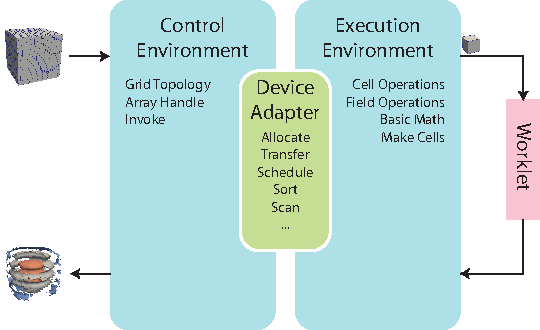
\includegraphics[width=\linewidth]{vtkm-framework}
  \caption{The basic VTK-m framework that allows device portability.}
  \label{fig:vtkm-framework}
\end{figure}

Mesh structures are definined using a flexible data model \cite{Meredith2012} in the control environment.
Based on the structure, the data are divided in small pieces, and the pieces are processed in parallel in the execution environment.

All of these aforementioned structural units are implemented with standard C++14 and are universal for any GPU device.
To achieve portability, VTK-m contains a device adapter that manages interaction with a variety of devices.
The entirety of VTK-m can be ported with a change to the device adapter.

The device adapter enables parallel execution using the data parallel primitive method \cite{Blelloch1990}.
Data parallel primitives allow algorithms to be implemented as a sequence of data parallel operations such as scan, sort, or reduce.
Early work explored how to implement scientific visualization using data parellel primitives \cite{Lo2012}.
To simplify the implementation further, VTK-m provides a layer of meta data parallel primitives \cite{Moreland2021} that are shown to be efficient during use.
